\documentclass{minimal}
\usepackage{tikz}
\usetikzlibrary{calc}

\begin{document}

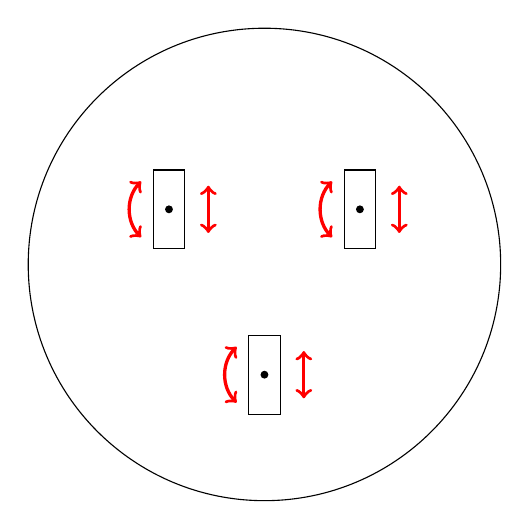
\begin{tikzpicture}[auto]
    \def\Aa{30} \def\Ab{150} \def\Ac{270}
    \def\R{1.4} \def\r{.5} \def\l{.3}
    \coordinate (o) at (0, 0);
    \coordinate (A) at ({\R * cos(\Aa)}, {\R * sin(\Aa)});
    \coordinate (B) at ({\R * cos(\Ab)}, {\R * sin(\Ab)});
    \coordinate (C) at ({\R * cos(\Ac)}, {\R * sin(\Ac)});
    \coordinate (roue) at (.2, .5);
    \coordinate (rot) at ({-\r/sqrt(2)}, {\r/sqrt(2)});
    \coordinate (caster) at (0, -1);

    \draw (o) circle (3);
    \fill (A) circle (.05);
    \fill (B) circle (.05);
    \fill (C) circle (.05);

    \draw ($ (A) - (roue) $) rectangle ($ (A) + (roue) $);
    \draw ($ (B) - (roue) $) rectangle ($ (B) + (roue) $);
    \draw ($ (C) - (roue) $) rectangle ($ (C) + (roue) $);
    \draw [<->, very thick, red] ($ (A) + (\r, \l) $) -- ($ (A) + (\r, -\l) $);
    \draw [<->, very thick, red] ($ (B) + (\r, \l) $) -- ($ (B) + (\r, -\l) $);
    \draw [<->, very thick, red] ($ (C) + (\r, \l) $) -- ($ (C) + (\r, -\l) $);
    \draw [<->, very thick, red] ($ (A) + (rot) $) arc (135:225:\r);
    \draw [<->, very thick, red] ($ (B) + (rot) $) arc (135:225:\r);
    \draw [<->, very thick, red] ($ (C) + (rot) $) arc (135:225:\r);
\end{tikzpicture}

\end{document}
